\chapter{Data Visualization}
\label{chap:dataviz}
Data visualization is a field that helps translate data and information into a graphical representation. The visual representation can help the reader understand the data story better. Especially large datasets can be hard to navigate and understand, and it is often important to make informed decisions. Data visualization is useful in many fields including network security \citep{shiravi2011survey}, money laundering \citep{singh2019anti}, improvement of services \cite{alharthi2017data}, and crime detection \citep{feng2019big}. A review of how data visualization can be useful in the medical field can be found in \cite{park2022impact} and \cite{aung2019leveraging}.

The graphical representation can make it easier to identify patterns, trends, and outliers. Relationships between datapoints can be represented by various plots depending on whether it is desirable to represent relationships or connections in a form of a network. Data visualization is closely related to human creativity \citep{dove2013using, li2018data}. 

Data visualization can be either static or interactive. The advantage of an interactive solution is that it allows the user to explore the data with various filters, highlighting possible subsets. A proof of concept of how switching plots from static to interactive can improve data exploration can be found in \cite{weissgerber2016static}. 

Data visualization is also an important element of data sharing, as it can be more engaging and memorable than other forms of data presentation. 

Data is visualized by mapping data and visual features, be it shape, size, or color. 

\paragraph{Use of color}
\label{sec:color}
Color is an important aspect of communication. According to the Commission Internationale de L'Eclairge, a color can be specified by using three dimensions: luminance, saturation, and hue \citep{wyszecki2000color}. This is especially important for people with color perception difficulties, as discussed later. More about color theory can be read in \cite{healey1996choosing}.
Color can be used in several ways:
\begin{itemize}
    \item To represent different data points or data groups
    \item To represent value of a feature such as elevation or saturation, whether the value is positive or negative
    \item To highlight information and draw attention
    \item To create contrast
    \item To create hierarchy
    \item To create aesthetic appeal and make information more engaging and memorable
\end{itemize}

However, color can also be used to mislead the consumer \citep{szafir2018good}, and the semantic meaning of color can be taken advantage of \citep{lin2013selecting}.

When designing a solution, it is important to focus on color accessibility. Colorblindness, which affects the visible spectrum of some people, affects about 8 percent of males and 0.5 of females of European ancestry. The most common type is the red-green colorblindness, however, other types can be found as well \citep{wong2011color}.

There are several ways one can make their tools more accessible to people with color perception difficulties.

\begin{itemize}
    \item Using other means of conveying information, such as shape or size or text
    \item Choosing high contrast color which can also be visible in monochromatic color schemes
    \item Creating an accessible color palette and avoiding colors that can cause difficulties
    \item Labeling data
\end{itemize}


\paragraph{Heatmap}
\label{sec:heatmap}
A heatmap is a 2D grid. In a heatmap, data is represented by mapping values to colors, making it easy to spot areas of high and low density. Another advantage of a heatmap is that the user can visualize large amounts of data in a small space. An example of a heatmap is shown in \ref{heatmapex}.
\begin{figure}[h!]
    \centering
    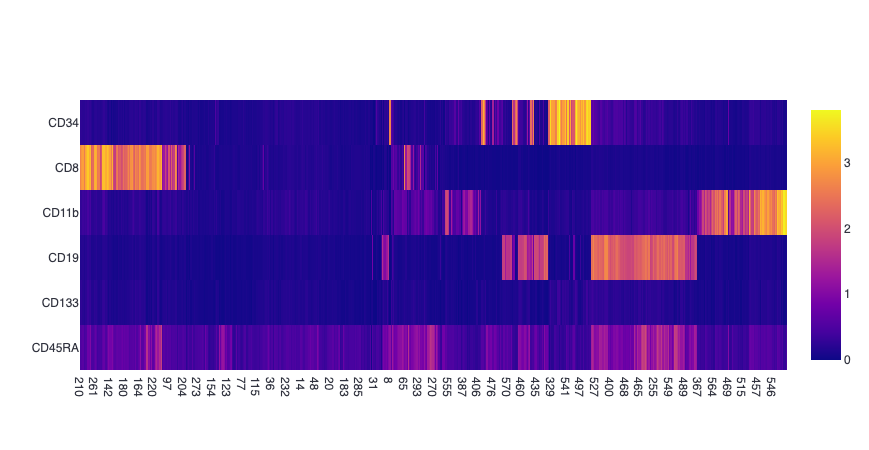
\includegraphics[width=0.9\textwidth]{Figures/heatmapex.png}
    \caption{An example of a heatmap}
    \label{fig:heatmapex}
\end{figure}

\paragraph{Dendrogram}
\label{sec:dendrogram}
A dendrogram, also known as a tree diagram or a tree map, is a 2D data representation that is designed to reveal the hierarchical structure of data. The use of dendrograms is popular in biology, where it can be useful for taxonomy \citep{calinski2014dendrogram} and other purposes \citep{lee2012persistent, rosolowsky2008structural}, and in other data clustering problems \cite{phipps1971dendrogram}.
The structure of a dendrogram is shown in \ref{fig:exdendr}. 

The data points are called leaf nodes, and it is the end nodes of the structure. Leaf nodes are linked together by branches, and branches are joined together in nodes. 

Clusters share the same upper nodes, and color can be used to highlight separate nodes, especially in dendrograms that show a lot of datapoints. The top of the dendrogram refers to the least specific grouping. 

Dendrograms can be obtained by a variety of grouping algorithms, including hierarchical clustering as described in \ref{sec:hierarchicalclustering}. 

\begin{figure}[h!]
    \centering
    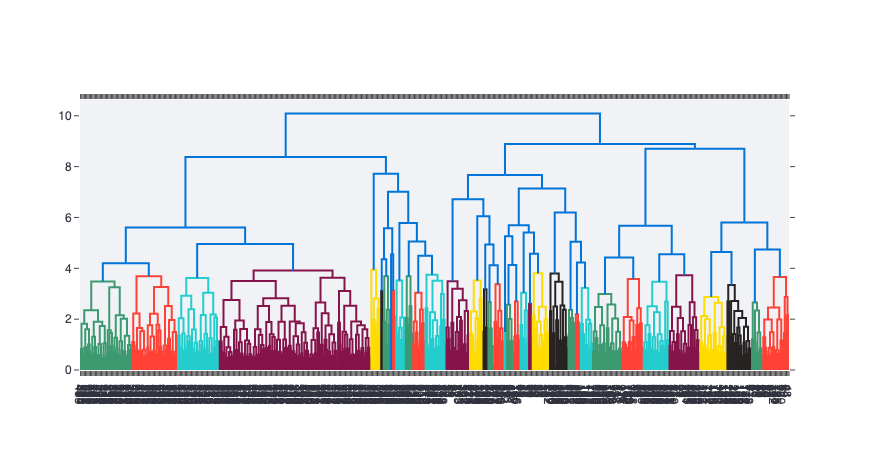
\includegraphics[width=0.9\textwidth]{Figures/dendrogramex.png}
    \caption{An example of a dendrogram}
    \label{fig:exdendr}
\end{figure}

\paragraph{Dimension Reduction}
\label{sec:dimred}
Dimension reduction is a method that can be used to plot high-dimensional data to low-dimensional space. Humans can comfortably plot in 2D and 3D. 

Some popular data reduction algorithms include the principal component analysis (PCA), t-Distributed Stochastic Neighbor Embedding (t-SNE), or uniform manifold approximation and projection (UMAP).

Each of the algorithms has its own merits and its own downfalls.

PCA is an unsupervised method based on linear combinations of original variables. It creates a new set which consists of of uncorrelated variables which capture variation in the original data. Thanks to the unsupervised nature, it can be used to explore datasets of unknown structures. It is also applicable to large datasets. However, it can struggle with datasets that have non-linear structure, is non normally distributed. PCA is also sensitive to scaling and work better on normalized data. It may also be difficult to interpret the meaning of the principal components. 

Unlike PCA, t-SNE is a non-linear technique, meaning it can work better with data that have underlying non-linear structure. The advantage for visualization is that it preserves the pairwise distances between data points. t-SNE can also identify outliers. However, it is more computationally expensive, especially as the number of dimensions grows. It is possible to fine tune the algorithm. 

UMAP is similar to t-SNE in many aspects. It aims to preserve local structure rather than global. UMAP can work well with outliers and can handle large datasets. It also scales well. UMAP requires some fine tuning and is not guaranteed to converge to a local minimum.

